\section{Atributo}
\label{sec:atributo}

Los atributos son los elementos utilizados en el standard UML para designar
propiedades que son inherentes a las clases, una vez instanciadas (las clases)
estos (los atributos) toman valor y ayudan al manejo de datos del objeto; El
lenguaje propuesto, permite el manejo de los atributos y algunas otras
cuestiones que están relacionadas con estos.

Teniendo en cuenta que el atributo tiene que estar definido dentro de otra
estructura del estándar UML, una clase.

A continuación un ejemplo con Director, para expresar medianamente el
funcionamiento del mismo:\\

\begin{displayquote}
	\texttt{Consigna}: \textit{se desea tener una clase que permita el manejo de
	información de una persona, la información a manejar es el nombre, apellido
	y DNI}.
\end{displayquote}

Lo cual se puede representar mediante un diagrama de clase de la siguiente manera:

\begin{figure}[H]
	\centering
	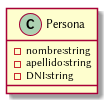
\includegraphics[width=.2\linewidth]{diagramas_clases/ej_diag_clase.png}
	\caption{Diagrama de Clase - representación de la consigna}
	\label{fig:ej_diag_clase.png}
\end{figure}

Teniendo esta información se puede armar un modelo en el lenguaje Director que
concuerde con estos requerimientos.

\textit{Dado a que por el momento unicamente se está tratando con los atributos
no se tendrá en cuenta la declaración de la clase \texttt{Persona} mencionada
en la consigna propuesta}.

\begin{lstlisting}[caption={Director - Modelado de atributos}, label=lst:atributo]
  ...
		private nombre:string
		private apellido:string
		private DNI:string
	...
\end{lstlisting}

Lo expuesto en el \texttt{Fragmento \ref{lst:atributo}}, demuestra
la capacidad del lenguaje de describir una serie de atributos con sus
respectivos metadatos (visibilidad y tipo); sin embargo, cabe destacar que
también se deja abierta la posibilidad de la futura implementación y
la compatibilización con funcionalidades relacionadas al Lenguaje de
Restricción de Objetos, puesto a que la adición de éstas
características automatizaría aún más el proceso de
desarrollo y permitiría el pase de modelo-a-código de manera mas sencilla.

Las características que se implementan compatibles funcionalidades brindadas
por OCL son las de modificadores para los atributos, estos modificadores ya
se mencionaron en la \texttt{Sección \ref{sec:palabrasreservadas}}.

Como ejemplo, se podrían aplicar algunas de estas cuestiones a lo implementado
en \texttt{Fragmento \ref{lst:atributo}} resultando lo siguiente:

\begin{lstlisting}[caption={Director - Modelao de atributos (con OCL)},
label=lst:atributo_restr]
  ...
		private nombre:string
		private apellido:string
		private DNI:string {@id, @readOnly, @unique}
	...
\end{lstlisting}

De esta forma, lo implementado en el \texttt{Fragmento
\ref{lst:atributo_restr}} brinda información como para que se pueda determinar
que el atributo DNI:
\begin{itemize}
	\item debe ser tratado como un identificador de la clase.
	\item debe ser de solo lectura, de este modo se deduce que no es necesaria la
		implementacion de un método \texttt{set} para el mismo.
	\item debe ser unico en el listado de personas, es decir, no se puede
		repetir.
\end{itemize}

Con esto, los resultados de la herramienta hacen que lo generado esté aun
más cerca al dominio en el que se esté trabajando.

A continuación se desarrollarán los componentes relacionados con lo Léxico y
Sintáctico para los atributos en sus respectivas secciones.

\subsubsection{Analizador Léxico}

El patrón a seguir para un atributo (sin establecer ningun metadato extra como
pueden ser las funcionalidades relacionadas con OCL mencionadas anteriormente) se describe en la siguiente expresión regular:

\begin{lstinputlisting}[language=Director, basicstyle=\footnotesize\ttfamily, caption={Regex - Atributo (sin
Modificadores)}, label=lstreatr]{regex/atributo/atributo_sin_modificadores.txt}

Dentro del lenguaje, este componente se puede ver gráficamente en
un autómata finito de la siguiente manera:

\begin{figure}[H]
	\centering
	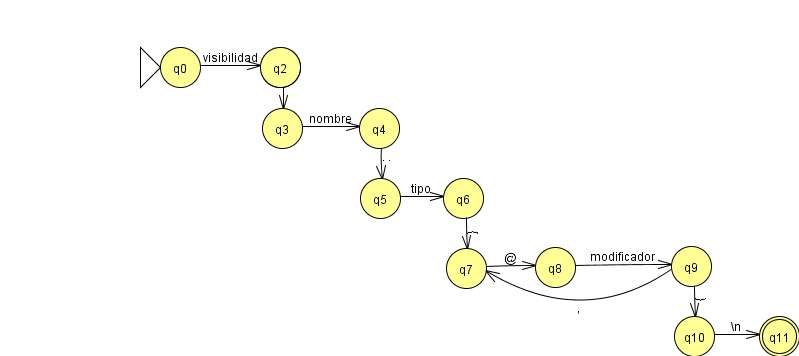
\includegraphics[width=.7\linewidth]{automatas_finitos/atributoDrt.png}
	\caption{Autómata finito - Atributo con restricciones de objeto}
	\label{fig:af_atr_modif}
\end{figure}

Luego de checkear los tokens que informan el tipo que tendrá el atributo se
deberá validar el uso de los modificadores que se le pueden adjuntar al
mismo, esto se describe en la siguiente expresion regular.

\begin{lstinputlisting} [basicstyle=\footnotesize, caption={Regex - Modificadores
  (Atributo)},
  label=lstreatrmodif]{regex/atributo/atributo_sin_modificadores.txt}

Esto permitirá las funcionalidades OCL que se vienen mencionando en cuanto a
los atributosi, además se puede definir un autómata para estos modificadores
de la siguiente manera:

\begin{figure}[H]
	\centering
	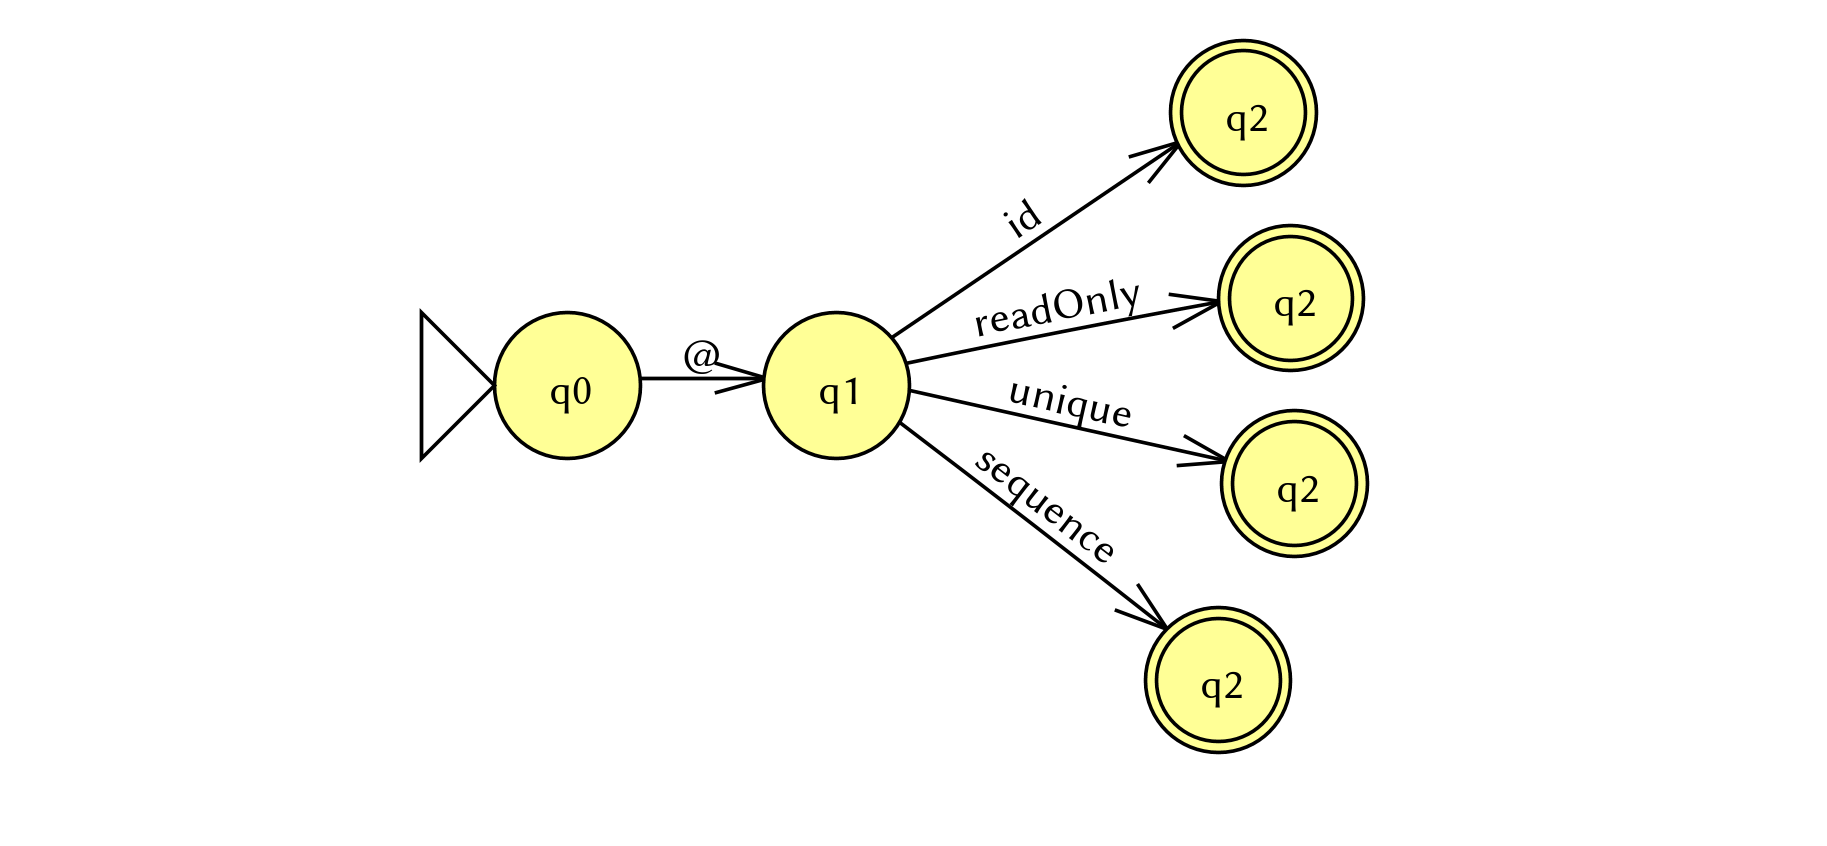
\includegraphics[width=.7\linewidth]{automatas_finitos/modificadores-drt.png}
	\caption{Autómata finito - Modificador para los atributos}
	\label{fig:af_atr_modif_OCL}
\end{figure}

\subsubsection{Analizador Sintáctico}

La definición de un atributo en cuanto a la gramática libre
de contexto según notacion BNF es la siguiente:

\begin{lstlisting}[caption={BNF - Atributo}, basicstyle=\footnotesize\ttfamily]
  <atributo> ::= <visibilidad> <nombre> ":" <tipo>
\end{lstlisting}

Se puede dejar expresado que el BNF, teniendo en cuenta la incorporación de lo
relacionado a la funcionalidad OCL (relacion directa con los fragmentos
\texttt{\ref{lstreatr}} y \texttt{\ref{lstreatrmodif}}), queda de la siguiente manera:

\begin{lstlisting}[caption={BNF - Atributo}, basicstyle=\ttfamily\footnotesize,
label=lst:bnf_atributo_restr]
		<atributo> ::= <visibilidad> <nombre> ":" <tipo>
		               "{" <modificadores> "}"
\end{lstlisting}

En donde \texttt{modificadores} es la pluralización de un \texttt{modificador}:

\begin{lstlisting}[basicstyle=\ttfamily\footnotesize]
	<modificadores> ::= <modificador> | <modificadores>
\end{lstlisting}

y \texttt{modificador} se define de la siguiente manera:

\begin{lstlisting}[language=Java, basicstyle=\footnotesize\ttfamily, label=lst:bnf_atributo_modif]
	<modificador> ::= @id | @readOnly | @unique | @sequence
\end{lstlisting}

\subsubsection{Derivaciones Atributo}

Para finalizar con la sección se puede armar un ejemplo con la definición de un
atributo con todas las características mencionadas y proceder a su análisis
mediante las Derivaciones y los Árboles Sintácticos. Para el ejemplo se
utilizará la siguiente declaración de un atributo:

\begin{lstlisting}
  EJEMPLO: public CUIT:string{@unique, @readOnly}
\end{lstlisting}

Las gramáticas libre de contexto para estas derivaciones se detallan en el
\texttt{Fragmento \ref{lst:bnf_atributo_restr}}.

Por cuestiones de espacio y de lo extenso de las derivaciones para los
componentes, se tomaron abreviaciones para algunos componentes, a continuación
se detalla el significado de cada una de ellos.

\begin{itemize}
  \item \textbf{V}: visibilidad
  \item \textbf{N}: nombre
  \item \textbf{SE}: simbolo especial
  \item \textbf{T}: tipo
  \item \textbf{MA}: modificador atributo
  \item \textbf{SM}: separador modificador
\end{itemize}

\begin{lstlisting}[basicstyle=\footnotesize\ttfamily, caption={Derivaciones -
Atributo}, label=deratr]
  comp-drt -> atributo
  atributo -> visibilidad nombre sim-esp tipo modificador
  atributo -> V N SE T sim-esp modif-atr sep-mod modif-atr sim-esp
  atributo -> public N SE T SE MA SM MA SE
  atributo -> public CUIT SE T SE MA SM MA SE
  atributo -> public CUIT: T SE MA SM MA SE
  atributo -> public CUIT: string SE MA SM MA SE
  atributo -> public CUIT: string{ MA SM MA SE
  atributo -> public CUIT: string{@unique SM MA SE
  atributo -> public CUIT: string{@unique, MA SE
  atributo -> public CUIT: string{@unique, @readOnly SE
  atributo -> public CUIT: string{@unique, @readOnly}
\end{lstlisting}

El arbol sintáctico para las derivaciones del \texttt{Fragmento \ref{deratr}}
es el siguiente:

\begin{figure}[H]
  \centering
  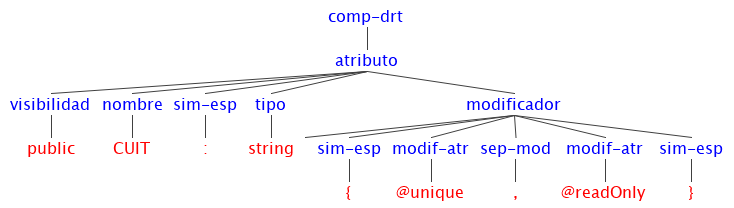
\includegraphics[width=.7\linewidth]{arboles_sintaxis/2_atributo.png}
  \caption{Árbol Sintáctico - Atributo}
  \label{as:atr}
\end{figure}
